% Background section
\subsection{Properties of Complex Systems}

\subsubsection{Structural Features: Near-decomposability and Scale-invariance}

Complex systems exhibit two foundational structural properties that enable their characteristic behaviors and provide the basis for our operadic approach.

\textbf{Near-decomposability} \citep{simon1962architecture} describes systems with subsystems that interact weakly externally while maintaining strong internal interactions. These systems display:

\begin{itemize}
    \item Stronger interactions within subsystems than between them
    \item Hierarchical organization across multiple levels
    \item Time-scale separation between internal and external interactions
\end{itemize}

Examples include cellular structures (organelles within cells, cells within tissues, tissues within organs, organs within organisms, etc.), ecosystems with loosely coupled niches, and modular software systems. Near-decomposability enables adaptation through independent subsystem evolution \citep{simon1996sciences} and creates the hierarchical levels across which system dynamics unfold.

\textbf{Scale-invariance} describes self-similar patterns appearing across different organizational levels, characterized by:

\begin{itemize}
    \item Statistical similarity at different observation scales
    \item Power-law distributions of system properties
    \item Absence of characteristic scales
\end{itemize}

This property manifests in branching patterns in biological systems, power-law distributions in scale-free networks etc. \citep{west2017scale, stanley1999scaling}. Scale-invariance emerges naturally in systems that grow through preferential attachment processes or self-organize into critical states.

\subsubsection{Dynamical Features: Phase Transitions and Emergence}

Phase transitions and emergence represent related dynamical phenomena that arise from the hierarchical and scale-invariant structures of complex systems.

\textbf{Phase transitions} occur when control parameters cross threshold values, causing qualitative changes in system properties. These transitions manifest as discontinuous shifts at critical points \citep{stanley1971phase}, displaying characteristic mathematical signatures: power-law scaling behaviors, critical exponents, and diverging correlation lengths \citep{newman2003structure, bak1987self}. In complex systems, phase transitions include ecosystem state shifts, opinion cascades in social networks, synchronization transitions in oscillator systems, financial market crashes, and percolation thresholds in networks.

\textbf{Emergence} describes the formation of properties at higher organizational levels not present in or predictable from individual components \citep{holland1998emergence, anderson1972more}. Anderson's "More is Different" principle emphasizes that complex systems require analysis beyond reductionist approaches. Examples include flocking behaviors in birds, intelligence in neural networks, consciousness from neuronal activity, and market dynamics in economies \citep{camazine2003self, haken1983synergetics}.

Phase transitions can be viewed as a specific type of emergence characterized by sudden, discontinuous changes, while other emergent phenomena may develop gradually or exist in steady states \citep{bar2013computability}. Both phenomena share common underlying mechanisms:

\begin{itemize}
    \item They arise from the hierarchical structures created by near-decomposability
    \item They propagate across scales following patterns enabled by scale-invariance
    \item They involve reorganization of compositional relationships between system components
    \item They manifest when local changes cascade to produce system-wide transformations
\end{itemize}

At critical points, fluctuations occur across all scales of the system as local changes propagate through hierarchical levels—a direct consequence of the near-decomposable, scale-invariant structure.

Our operadic framework models these phenomena by tracking compositional relationships between components across scales. This approach complements traditional statistical methods \citep{stanley1999scaling, goldenfeld1992lectures} by focusing explicitly on how compositional structures reorganize during transitions, providing insights into the mechanisms driving phase transitions and emergent behaviors.

\subsection{Modeling Phase Transitions and Emergence}

\subsubsection{Physical Models}

In physics, phase transitions are often modeled using statistical mechanics, where the system's behavior is described in terms of energy, entropy, and temperature \citep{stanley1971phase, kadanoff2000statistical}. The Ising model, Potts model, and percolation theory are classic examples of physical models used to study phase transitions \citep{onsager1944crystal, stauffer2018introduction}. These models capture the interactions between individual components and the emergence of collective behavior at critical points \citep{binney1992theory}. They, however, have limitations in capturing the complexity of real-world systems, such as biological, social, and technological networks but tend to be more mathematically tractable for detailed analysis \citep{newman2011structure}.

\subsubsection{Network Models}

Networks have been used since the early 20th century to model complex systems, representing entities as nodes and interactions as edges \citep{watts1998collective, barabasi1999emergence}. Formally, a network is represented as a graph $G = (V, E)$ where $V$ is a set of vertices (nodes) and $E \subseteq V \times V$ is a set of edges (links). For directed networks, edges are ordered pairs $(u, v) \in E$ indicating a directed relationship from node $u$ to node $v$. For undirected networks, edges are unordered pairs $\{u, v\} \in E$.

The structure of a network can be represented by its adjacency matrix $A$, where:
\begin{equation}
A_{ij} =
\begin{cases}
1 & \text{if } (i,j) \in E \text{ (or } \{i,j\} \in E \text{ for undirected graphs)} \\
0 & \text{otherwise}
\end{cases}
\end{equation}

For weighted networks, $A_{ij}$ represents the strength of the connection between nodes $i$ and $j$. Several metrics characterize network properties:

\begin{itemize}
    \item \textbf{Degree distribution} $P(k)$: The probability that a randomly selected node has $k$ connections
    \item \textbf{Clustering coefficient} $C_i$: For a node $i$ with $k_i$ neighbors, $C_i = \frac{2e_i}{k_i(k_i-1)}$ where $e_i$ is the number of links between the neighbors
    \item \textbf{Path length} $d(i,j)$: The minimum number of edges traversed to reach node $j$ from node $i$
    \item \textbf{Betweenness centrality} $B(v)$: $B(v) = \sum_{s \neq v \neq t} \frac{\sigma_{st}(v)}{\sigma_{st}}$ where $\sigma_{st}$ is the number of shortest paths from $s$ to $t$ and $\sigma_{st}(v)$ is the number of those paths passing through $v$
\end{itemize}

These properties can be used to classify networks into different categories, such as \textbf{scale-free}, \textbf{small-world}, and \textbf{random networks} \citep{barabasi1999emergence, watts1998collective}.

\begin{figure}[htbp]
    \centering
    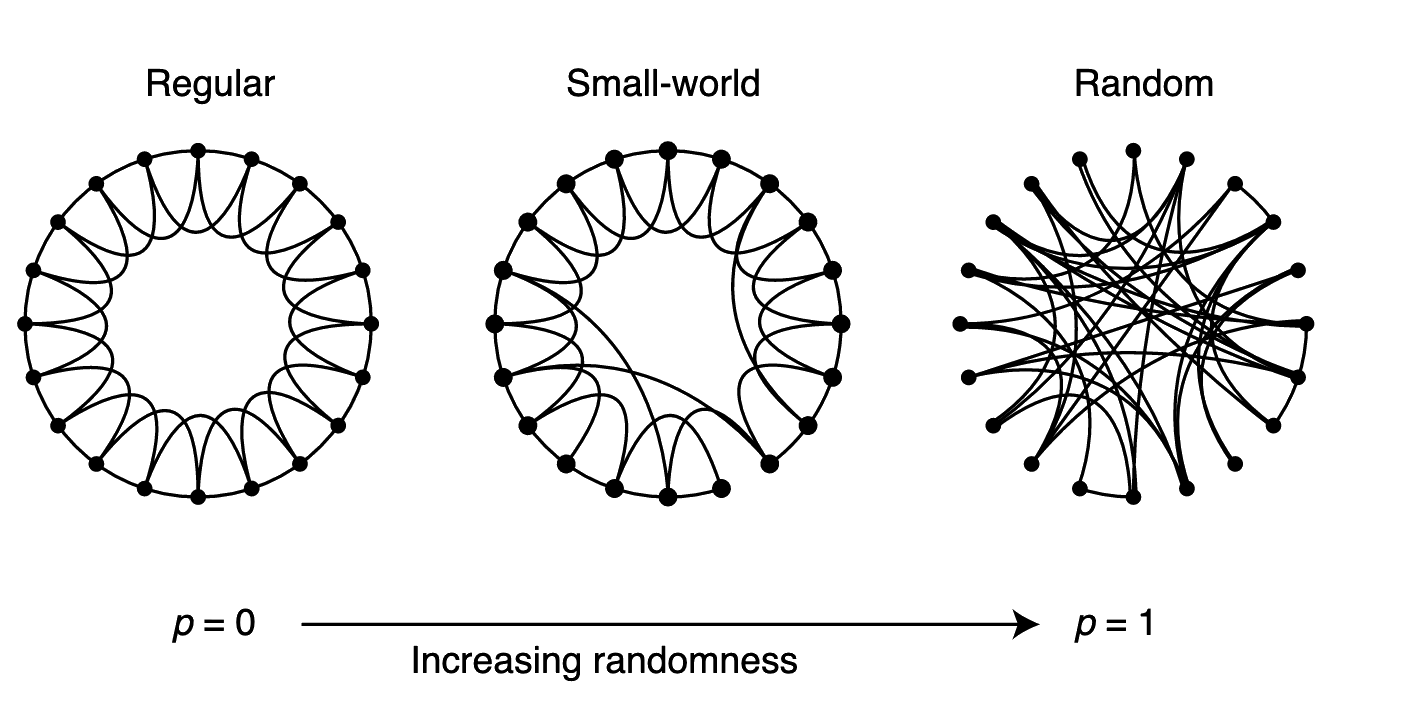
\includegraphics[width=0.8\textwidth]{figures/networks.png}
    \caption{Small-world network model illustration showing the transition from regular to random networks. \citep{watts1998collective}. A regular network transitions to a small-world network by rewiring a fraction of the edges, leading to a significant reduction in the average path length while maintaining high clustering.}
    \label{fig:small_world}
\end{figure}

Critical phenomena in networks, such as phase transitions, often manifest through sudden changes in global network properties. For instance, the emergence of a giant connected component in random networks occurs at a critical probability $p_c = \frac{1}{N}$, where $N$ is the number of nodes \citep{erdos1960evolution}.

\begin{figure}[htbp]
    \centering
    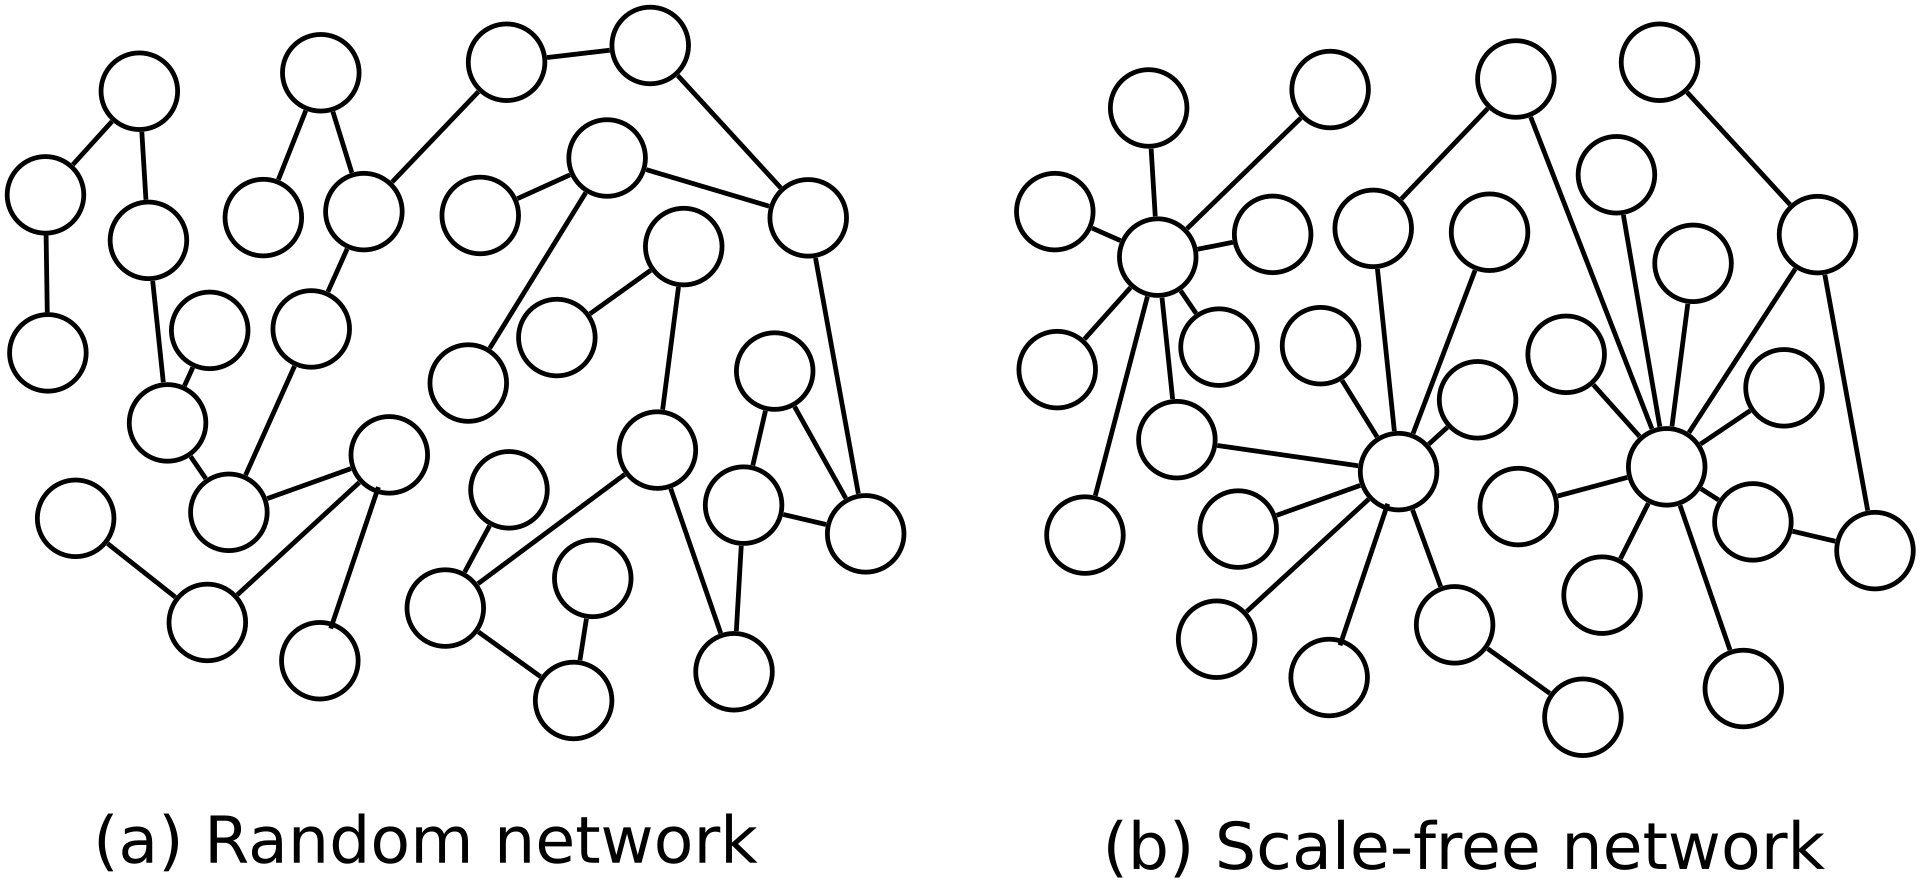
\includegraphics[width=0.8\textwidth]{figures/scalefree.png}
    \caption{Visual comparison between random and scale-free networks. \citep{wikipedia2023scalefree}. Notice the presence of hubs in the scale-free network, which are absent in the random network.}
    \label{fig:small_world}
\end{figure}

\begin{table}[htbp]
    \centering
    \begin{tabular}{p{2.5cm}|p{3cm}|p{3cm}|p{3cm}}
        \hline
        \textbf{Network Type} & \textbf{Degree Distribution} & \textbf{Clustering Coefficient} & \textbf{Average Path Length} \\
        \hline
        Random Networks & Poisson distribution $P(k) \sim \frac{\lambda^k e^{-\lambda}}{k!}$ & Low ($C \sim \frac{p}{N}$) & Short ($L \sim \frac{\ln N}{\ln \langle k \rangle}$) \\
        \hline
        Regular Lattices & Constant degree & High (locally clustered) & Long ($L \sim N^{1/d}$) \\
        \hline
        Small-World Networks & Similar to random networks & High ($C \gg C_{random}$) & Short ($L \approx L_{random}$) \\
        \hline
        Scale-Free Networks & Power law $P(k) \sim k^{-\gamma}$ & Hierarchical clustering & Very short (ultra-small world) \\
        \hline
        Hierarchical Networks & Power law & Hierarchical ($C(k) \sim k^{-1}$) & Short \\
        \hline
        Modular Networks & Varies & High within modules, low between modules & Long between modules, short within modules \\
        \hline
    \end{tabular}
    \caption{Comparison of Different Network Types and Their Characteristics.
        \textbf{Notation:}\\
        $P(k)$ = probability that a randomly selected node has $k$ connections (degree distribution)\\
        $k$ = node degree (number of connections)\\
        $\langle k \rangle$ = average degree across the network\\
        $C$ = clustering coefficient (probability that two neighbors of a node are connected)\\
        $C(k)$ = clustering coefficient for nodes with degree $k$\\
        $L$ = average shortest path length between any two nodes\\
        $N$ = total number of nodes in the network\\
        $p$ = probability of connection between any two nodes (in random networks)\\
        $d$ = dimension of the lattice (for regular networks)\\
        $\gamma$ = power-law exponent (typically $2 < \gamma < 3$ for scale-free networks)}
    \label{tab:network_types}
\end{table}

Network models have been successful in capturing the structure and dynamics of a wide range of systems, including social networks, biological networks, and technological networks \citep{newman2003structure, albert2002statistical, strogatz2001exploring}. Networks are both a mathematically rigorous framework as well as intuitive and visually appealing, making them a popular choice for modeling complex systems \citep{newman2010networks}. Networks can capture the emergence of collective behavior through the study of network motifs, community structure, and dynamical processes on networks \citep{milo2002network, fortunato2010community, barrat2008dynamical}, and has attracted significant attention in recent years \citep{barabasi2016network}.

\subsubsection{From Networks to Simplicial Complexes}

\begin{figure}[htbp]
    \centering
    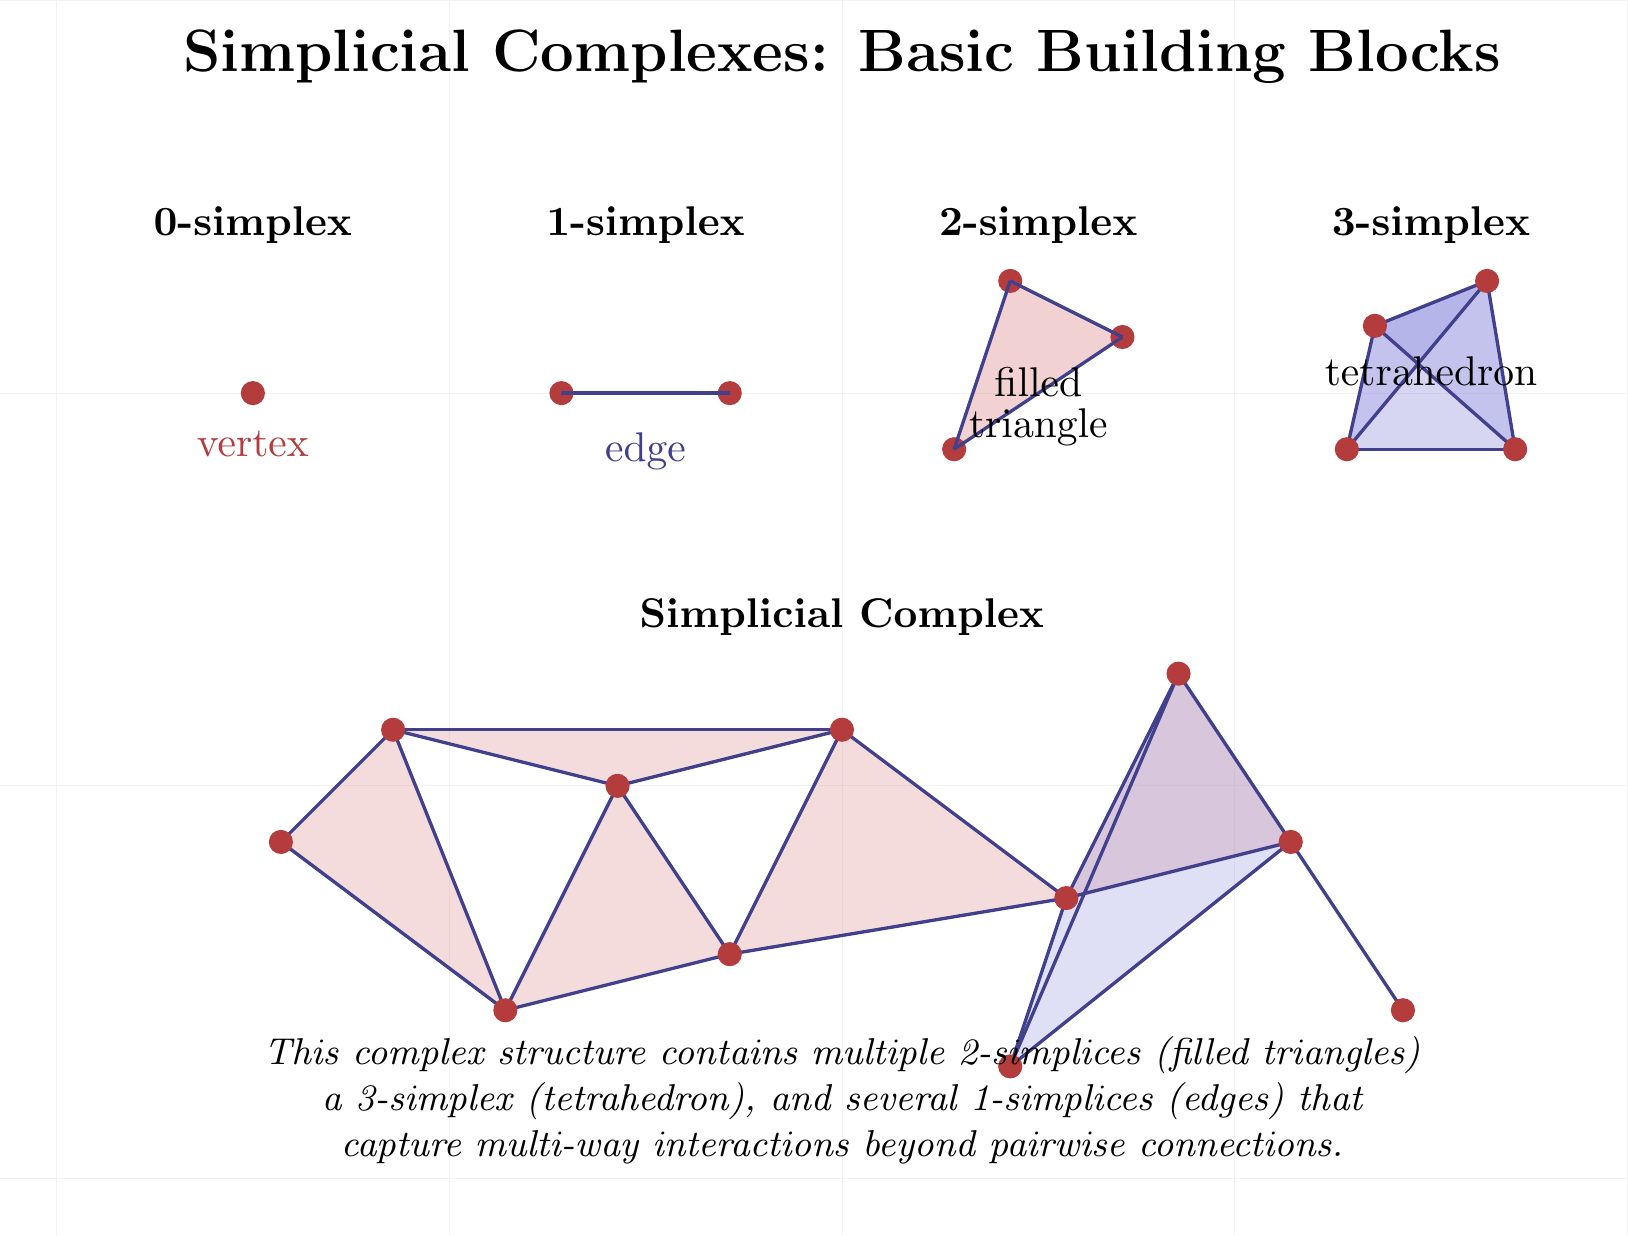
\includegraphics[width=\textwidth]{figures/simplicial_complexes-1.png}
    \caption{Visual representation of simplicial complexes. The top row shows individual simplices of different dimensions (0-simplex, 1-simplex, 2-simplex, and 3-simplex). The bottom part shows a more complex simplicial complex with multiple 2-simplices (filled triangles), a 3-simplex (tetrahedron), and connecting 1-simplices (edges) that capture multi-way interactions beyond pairwise connections.}
    \label{fig:simplicial_complexes}
\end{figure}

Simplicial complexes generalize networks by incorporating higher-order interactions. Simplicial complexes can be thought of as triangles of various dimensions - vertices (0-simplices), edges (1-simplices), triangles (2-simplices), tetrahedra (3-simplices), and so on \citep{petri2014homological} connected together either via shared vertices, edges, or faces.

Formally, a simplicial complex $K$ on a vertex set $V$ is a collection of subsets of $V$ (called simplices) such that:
\begin{itemize}
    \item For every vertex $v \in V$, $\{v\} \in K$ (0-simplex)
    \item If $\sigma \in K$ and $\tau \subset \sigma$, then $\tau \in K$ (closure property)
\end{itemize}

A $k$-simplex $\sigma = [v_0, v_1, ..., v_k]$ represents an interaction between $k+1$ vertices. For example:
\begin{itemize}
    \item A 0-simplex is a vertex
    \item A 1-simplex is an edge (pairwise interaction)
    \item A 2-simplex is a filled triangle (three-way interaction)
    \item A 3-simplex is a solid tetrahedron (four-way interaction)
    \item and so on
\end{itemize}

Several researchers have successfully applied simplicial complexes to model complex systems. \citet{petri2014homological} used simplicial complexes to analyze brain functional networks, revealing topological structures that correlate with cognitive states. \citet{giusti2016two} demonstrated how simplicial complexes can capture neural coding schemes beyond what traditional network models could represent. \citet{sizemore2018importance} showed how clique topology in neural systems provides insights into brain development and function.

While simplicial complexes offer significant advantages over traditional networks, they have inherent limitations:
\begin{itemize}
    \item They are \textit{undirected}, with no natural way to represent asymmetric interactions
    \item \textit{Temporal dynamics} are challenging to model in simplicial complexes
\end{itemize}
